\documentclass[mathserif,t]{beamer}
%\usepackage{Sweave}                                                       
\usepackage{amssymb,bm,mathtools,amsmath}                                                      
\usepackage{graphicx,caption,float}
\usepackage[UKenglish]{isodate} % for: \today                             
\cleanlookdateon                % for: \today                             

\def\wl{\par \vspace{\baselineskip}\noindent}                             
\def\beginmyfig{\begin{figure}[ht]\begin{center}}                          
\def\endmyfig{\end{center}\end{figure}}                                   

\def\prodl#1#2#3{\prod\limits_{#1=#2}^{#3}}                               
\def\suml#1#2#3{\sum\limits_{#1=#2}^{#3}}                                 
\def\ds{\displaystyle}                                                    
\def\tbf#1{\textbf{#1}}
\def\inv{^{\raisebox{.2ex}{$\scriptscriptstyle-1$}}}
\def\pm{^{\raisebox{.2ex}{$\scriptscriptstyle\prime$}}}

% My Beamer Stuff
  \geometry{vmargin=0.3in} % Formating the top bar
  \newcommand{\m}[1]{\mathbf{\bm{#1}}} % Serif bold math
  %\beamertemplatenavigationsymbolsempty % To get rid of navigation bar

  % My Color Stuff
  \usepackage{xcolor} % http://en.wikibooks.org/wiki/LaTeX/Colors
                      % http://latexcolor.com/
    \definecolor{grey}{rgb}{0.15, 0.15, 0.15} % Sets default color. CHANGE THIS!
    \definecolor{pumpkin}{rgb}{1.0, 0.46, 0.09}
    \definecolor{darktan}{rgb}{1.0, 0.66, 0.07}
    \definecolor{coral}{rgb}{1.0, 0.5, 0.31}
    \pagecolor{grey} % Sets the bar color.

  \def\mylitecolor{coral}           % Bullet Color.       CHANGE THIS!
  \def\mycolor{\color{pumpkin}}     % Frame Title Color.  CHANGE THIS!
  \def\mydarkcolor{\color{darktan}} % Figure Color.       CHANGE THIS!
    \def\frametitle#1{\vspace{-.32in{\mycolor\textbf{#1}}}}
    \setbeamercolor{itemize item}{fg=\mylitecolor}
    \setbeamercolor{enumerate item}{fg=\mylitecolor}
    \setbeamercolor{itemize subitem}{fg=\mylitecolor}
    \setbeamercolor{itemize subsubitem}{fg=\mylitecolor}
    \setbeamercolor{title}{fg=\mylitecolor}
    %\setbeamercolor{figure}{fg=\mylitecolor}

    \usepackage[T1]{fontenc}
    \DeclareCaptionFont{figcol}{\mydarkcolor} 
    \captionsetup{
      labelfont={bf,figcol},
      %textfont={green}
    }

  %% my title:                                                               
  %\title[short title]{long title}
  %\logo{\includegraphics[width=1cm,height=1cm,keepspectration]{logo.pdf}
  %\author[Arthur Lui]{Arthur Lui}
  %\institute[Brigham Young University]{
  %  Department of Statistics\\
  %  Brigham Young University
  %}

%%%%%%%%%%%%%%%%



\begin{document}
% My Title: {
  \def\mytitle{\textbf{Predicting Germination Rates of Different Tulip
                       Populations at Various Chilling Times}}
  \title[Tulips]{\mytitle}
  \author[Arthur Lui]{Arthur Lui}
  \institute{
    Department of Statistics\\
    Brigham Young University
  } \frame{\titlepage}
%}

\frame{
  \frametitle{Tulips in the Netherlands}
  \beginmyfig
    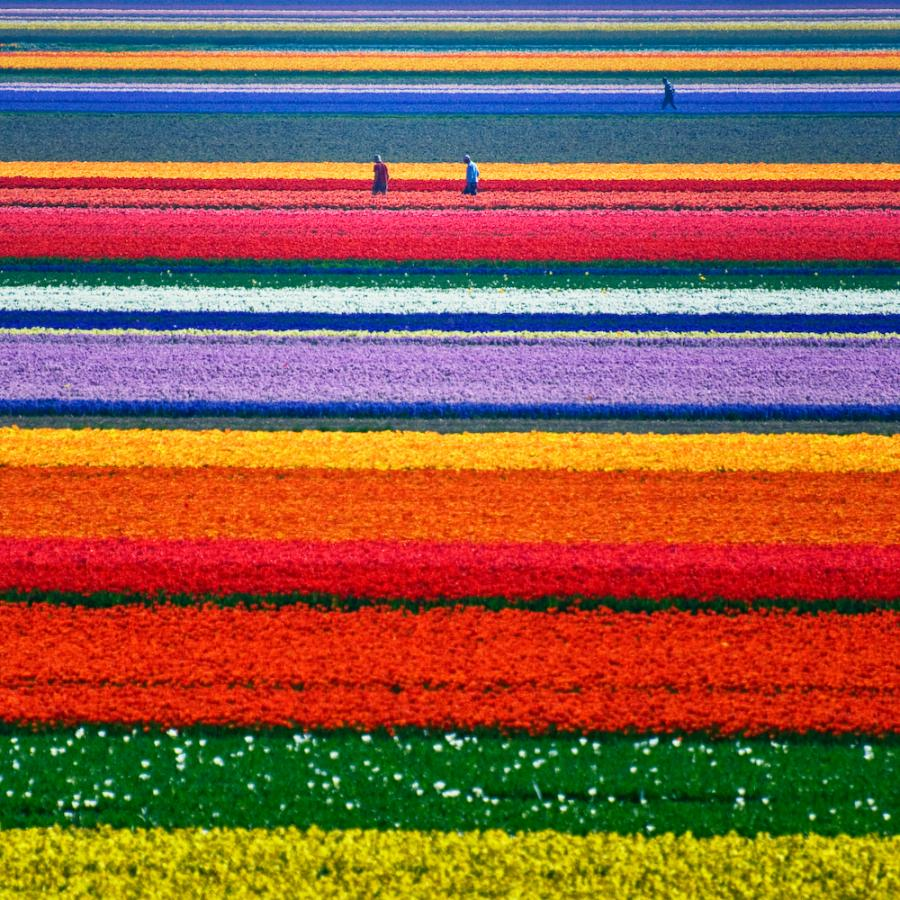
\includegraphics[scale=.22]{../../images/tulipsfieldsinholland6.jpg}
    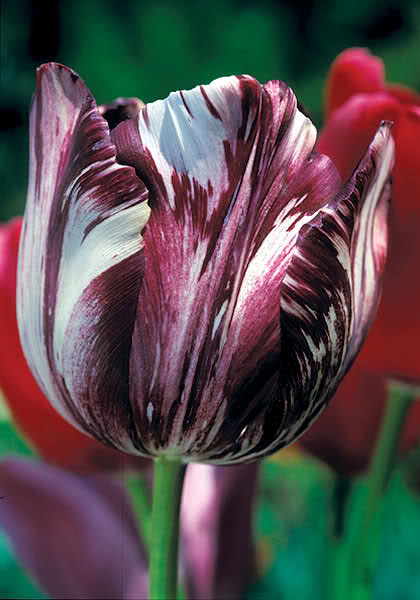
\includegraphics[scale=.22]{../../images/viceroy.jpg}
    \caption{Tulips popularized in the sixteenth century in Holland. During the 
             tulipomania, a viceroy tulip (right) bulb could be exchanged for a basket
             of goods, some furniture, and some live stock.}
  \endmyfig
}

\frame{
  \frametitle{Raw Data}
  \beginmyfig
    \includegraphics[scale=.22]{../../images/rawData.pdf}
    \vspace{-2mm}
    \caption{Germination rates of each population of tulips by chilling times
             (weeks)}
  \endmyfig
}

\frame{

}

\frame{
  \frametitle{Results}
  \beginmyfig
    \includegraphics[scale=.22]{../../images/chilleffect.pdf}
    \vspace{-2mm}
    \caption{Predicted germination rates of each population of tulips by
             chilling times (weeks)}
  \endmyfig
}

\end{document}
